\documentclass[aspectratio=169,11pt]{beamer}
\usepackage[utf8]{inputenc}
\usepackage[T1]{fontenc}
\usepackage{lmodern}
\usepackage{amsmath}
\usepackage{booktabs}
\usepackage{array}
\usepackage{graphicx}
\usepackage{caption}
\graphicspath{{slide_image/}}
\usepackage[authoryear,square]{natbib}
\setcitestyle{aysep={,}}
\newcommand{\RandomSample}{0.70}

\newcommand{\RandomGreedy}{1.77}

\newcommand{\RandomNoisy}{0.70}

\newcommand{\ProbabilitySample}{72.60}

\newcommand{\ProbabilityGreedy}{81.03}

\newcommand{\ProbabilityNoisy}{1.73}

\newcommand{\MarginSample}{71.57}

\newcommand{\MarginGreedy}{80.47}

\newcommand{\MarginNoisy}{2.90}

\newcommand{\EntropySample}{72.63}

\newcommand{\EntropyGreedy}{81.13}

\newcommand{\EntropyNoisy}{3.93}

\newcommand{\AdaptiveGain}{71.90}

\newcommand{\AdaptiveGainCI}{$[69.73,74.07]$}

\newcommand{\MainResultsRows}{Random & 0.70 & 51.06 \\
Probability & 72.60 & 89.69 \\
Margin & 71.57 & 89.38 \\
Entropy & 72.63 & 89.71 \\}

\newcommand{\PerSeedRows}{Random & 1.7 & 2.0 & 1.6 & 0.8 & 0.9 & 0.4 \\
Probability & 81.9 & 80.5 & 80.7 & 73.7 & 72.4 & 71.7 \\
Margin & 80.6 & 80.6 & 80.2 & 72.8 & 71.5 & 70.4 \\
Entropy & 81.5 & 81.0 & 80.9 & 73.8 & 73.4 & 70.7 \\}

\newcommand{\DigitChangeRows}{Random & 1.77 & 0.70 & -1.07 & $[-1.63,-0.53]$ \\
Probability & 81.03 & 72.60 & -8.43 & $[-9.67,-7.20]$ \\
Margin & 80.47 & 71.57 & -8.90 & $[-10.20,-7.63]$ \\
Entropy & 81.13 & 72.63 & -8.50 & $[-9.73,-7.30]$ \\}

\newcommand{\NoiseRows}{Random & 0.70 & 0.70 & +0.00 & $[0.00,0.00]$ \\
Probability & 72.60 & 1.73 & -70.87 & $[-73.03,-68.67]$ \\
Margin & 71.57 & 2.90 & -68.67 & $[-70.90,-66.40]$ \\
Entropy & 72.63 & 3.93 & -68.70 & $[-70.87,-66.50]$ \\}

\newcommand{\CheckpointRows}{\texttt{harry-100k} & 0.43 & 30.83 & 30.43 & 30.90 \\
\texttt{harry-500k} & 0.87 & 41.37 & 41.33 & 41.77 \\
\texttt{harry-combined} & 0.67 & 57.83 & 55.87 & 57.33 \\
\texttt{harry-hard} & 2.30 & 78.10 & 78.57 & 78.63 \\
DiT & 1.77 & 81.03 & 80.47 & 81.13 \\}

\newcommand{\ContrastRows}{Margin minus probability & -1.03 & $[-1.83,-0.23]$ \\
Entropy minus probability & +0.03 & $[-0.83,0.90]$ \\}

\newcommand{\CellAPeak}{0.55}

\newcommand{\CellAMargin}{0.11}

\newcommand{\CellAEntropy}{0.74}

\newcommand{\CellBPeak}{0.52}

\newcommand{\CellBMargin}{0.46}

\newcommand{\CellBEntropy}{1.69}

\usetheme{Madrid}
\definecolor{ink}{HTML}{233346}
\definecolor{muted}{HTML}{5C6A78}
\definecolor{probability}{HTML}{2675AF}
\definecolor{margin}{HTML}{D27C2C}
\definecolor{entropy}{HTML}{2E8B78}
\setbeamercolor{structure}{fg=ink}
\setbeamercolor{palette primary}{bg=ink,fg=white}
\setbeamercolor{frametitle}{bg=ink,fg=white}
\setbeamercolor{title}{bg=ink,fg=white}
\setbeamercolor{normal text}{fg=ink}
\setbeamerfont{frametitle}{series=\bfseries}
\setbeamersize{text margin left=0.6cm,text margin right=0.6cm}
\setbeamertemplate{navigation symbols}{}
\setbeamertemplate{footline}[frame number]
\setbeamertemplate{bibliography item}[text]
\setbeamertemplate{itemize items}[circle]
\setbeamertemplate{title page}[default][rounded=false,shadow=false]
\newcommand{\condition}[1]{\par\smallskip{\scriptsize\color{muted}#1\par}}
\newcommand{\takeaway}[1]{\par\medskip\textbf{#1}\par}
\title[Token ordering in MDMs]{Investigating Token Ordering Strategies\\in Masked Diffusion Models}
\author{Paul Bouchaud \and Arthur Djevahirdjian}
\institute{Generative AI project}
\date{}
\begin{document}

\begin{frame}
    \titlepage
\end{frame}


\begin{frame}{Discrete data generation : ARMs vs MDMs}
    \begin{itemize}
        \item[] \textbf{Autoregressive models} (ARM): generate tokens from left to right
        \bigskip
        \item[] \textbf{Masked diffusion models} (MDM): unmask tokens in no particular order.
    \end{itemize}
    \bigskip
    \begin{figure}
        \centering
        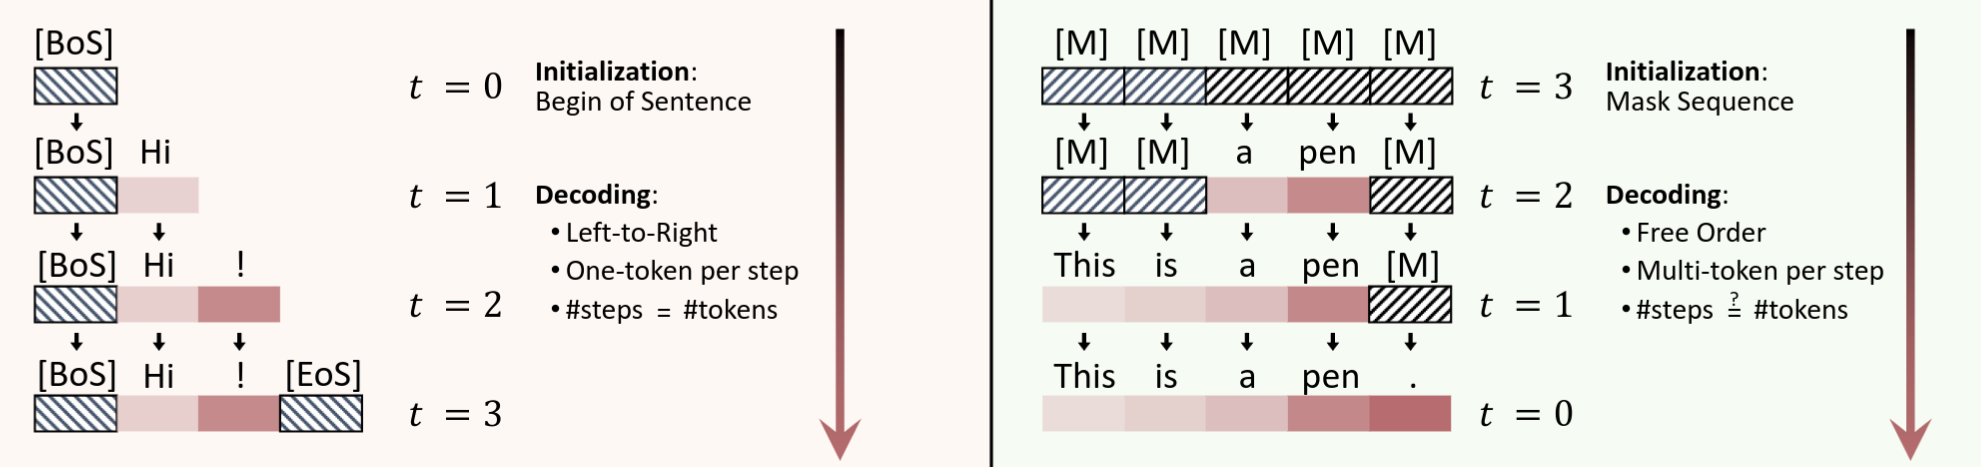
\includegraphics[width=0.9\textwidth]{slide_image/arm_mdm.png}
        \caption*{Source: Runpeng Yu, Qi Li, and Xinchao Wang. 2025. Discrete diffusion in large language and multimodal models: A survey.}
    \end{figure}
\end{frame}


\begin{frame}{Why study token ordering in masked diffusion?}
    \begin{columns}[T,onlytextwidth]
        \begin{column}{0.47\textwidth}
            Why move beyond ARM?\par
            Left-to-right order fits text.\par\medskip
            Sudoku and other reasoning tasks may have a different useful order for each instance.
        \end{column}
        \begin{column}{0.47\textwidth}
            What does MDM trade?\par
            It can reveal tokens in many orders.\par\medskip
            Random masking also makes it learn many difficult prediction problems.
        \end{column}
    \end{columns}
    \bigskip
    \takeaway{Paper's question: can a good decoding order use this flexibility to avoid hard predictions?}
    \condition{Kim et al. (2025), \emph{Train for the Worst, Plan for the Best}. }
\end{frame}


\begin{frame}{Decoding makes two separate decisions}
    \begin{center}
        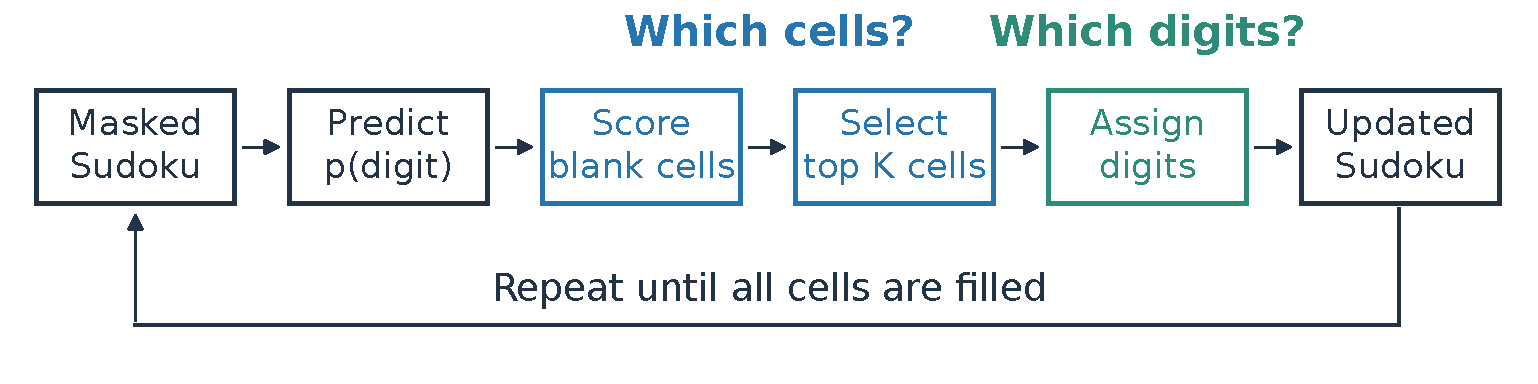
\includegraphics[width=\linewidth]{decoding_pipeline.pdf}
    \end{center}
    \begin{columns}[T,onlytextwidth]
        \begin{column}{0.48\textwidth}
            \textcolor{probability}{\textbf{Which cells?}}
            \par Random, probability or margin.
        \end{column}
        \begin{column}{0.48\textwidth}
            \textcolor{entropy}{\textbf{Which digits?}}
            \par Categorical sampling.
        \end{column}
    \end{columns}
    \takeaway{Selected cells use predictions from the same forward pass.}
    \condition{Previously revealed cells remain fixed. Solutions are used only for evaluation.}
\end{frame}

\begin{frame}{The results shown in the paper}
    \begin{itemize}
        \item \textbf{Random masking} leads to having to solve an untractable amount of problems.
        \item Using \textbf{top probability} or \textbf{top margin} improves solving accuracy. 
        \item \textbf{Top margin} performs better than \textbf{top probability}.
        \item These strategies allow \textbf{MDMs} to outperform \textbf{ARMs} in solving logic games like sudoku.
    \end{itemize}
    \bigskip
    Our additional hypothesis:
    \begin{itemize}
        \item Using a \textbf{lowest entropy} strategy can lead to better results than top margin 
    \end{itemize}
\end{frame}

\begin{frame}{Confidence scores capture different kinds of certainty}
    \begin{columns}[T,onlytextwidth]
        \begin{column}{0.46\textwidth}
            \small
            \textbf{Random:} uniform random cell scores.
            \medskip

            \textcolor{probability}{\textbf{Maximum probability:}} strongest digit.
            \[s_{\mathrm{prob}}(i)=p_i^{(1)}.\]
            \textcolor{margin}{\textbf{Margin:}} separation of the top two.
            \[s_{\mathrm{margin}}(i)=p_i^{(1)}-p_i^{(2)}.\]
            \textcolor{entropy}{\textbf{Lowest entropy:}} concentration of all digits.
            \[s_{\mathrm{entropy}}(i)=\sum_{j=1}^{9}p_i(j)\log p_i(j).\]
        \end{column}
        \begin{column}{0.50\textwidth}
            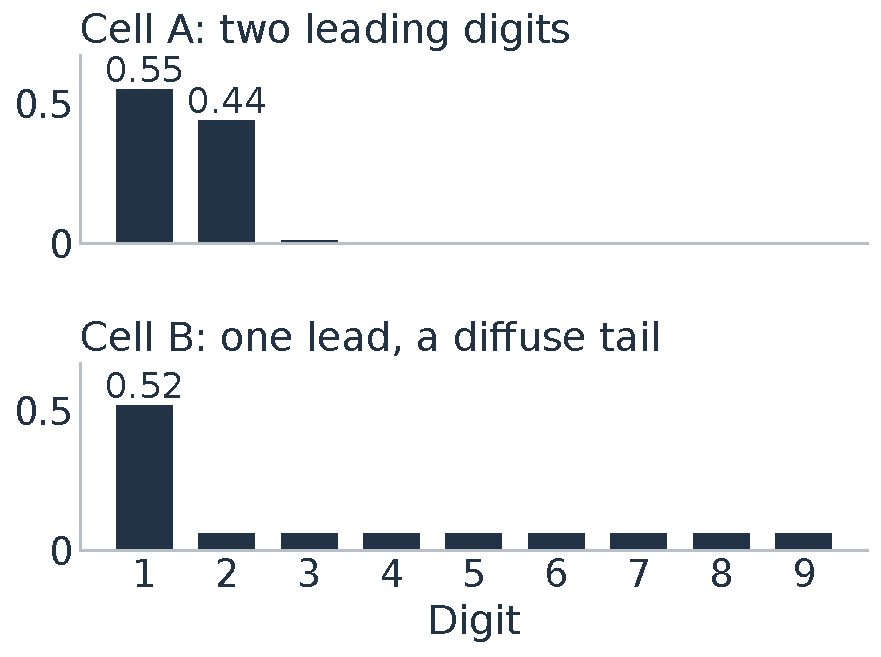
\includegraphics[width=\linewidth]{score_distributions.pdf}
            \small Probability and entropy prefer A. Margin prefers B.
        \end{column}
    \end{columns}
\end{frame}

\begin{frame}{All ordering rules receive the same solving budget}
    \begin{columns}[T,onlytextwidth]
        \begin{column}{0.48\textwidth}
            \textbf{Data and models}
            \begin{itemize}
                \item 1,000 fixed standard-test puzzles from a 100,000-puzzle release.
                \item Main model: frozen 1.28M-parameter DiT.
                \item Additional models: four frozen 806k-parameter encoder checkpoints.
            \end{itemize}
        \end{column}
        \begin{column}{0.48\textwidth}
            \textbf{Decoding and evaluation}
            \begin{itemize}
                \item Seeds 0, 1, 2. Batches of 32.
                \item Up to 50 steps, with shared binomial reveal counts.
                \item Exact puzzle accuracy, averaged over seeds.
            \end{itemize}
        \end{column}
    \end{columns}
\end{frame}

\begin{frame}{Adaptive ordering raises accuracy from 0.7\% to about 72.6\%}
    \begin{center}
        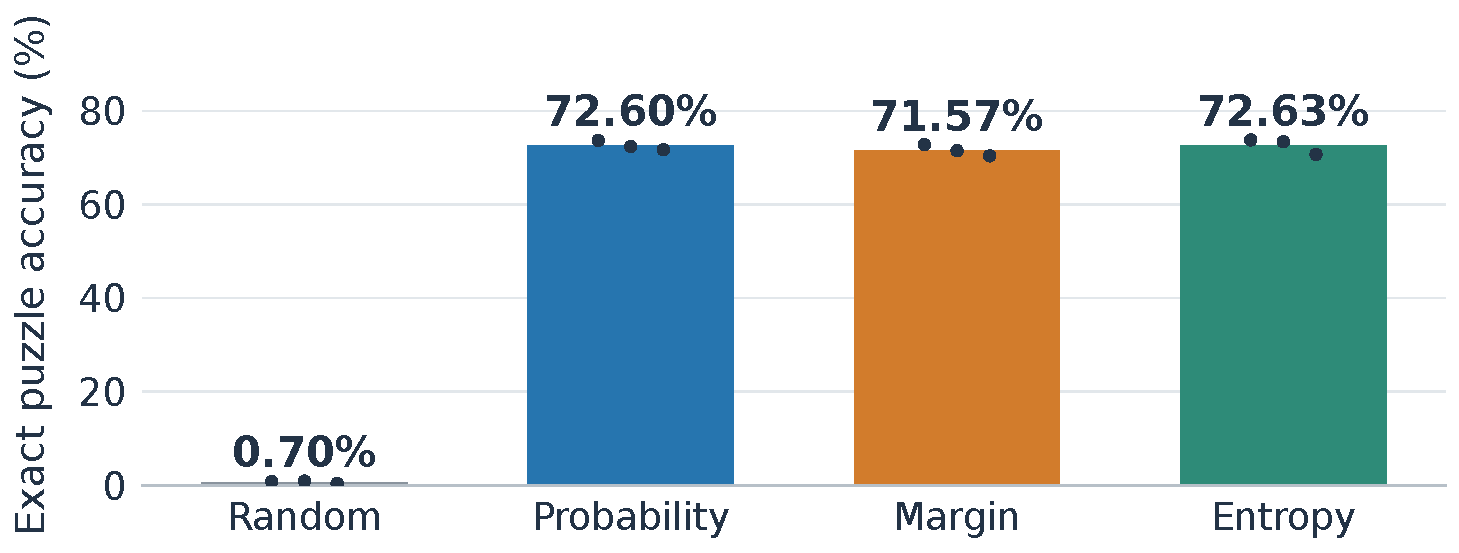
\includegraphics[width=0.96\linewidth,height=0.61\textheight,keepaspectratio]{sampled_accuracy.pdf}
    \end{center}
    \takeaway{Probability beats random by \AdaptiveGain\ percentage points.}
\end{frame}

\begin{frame}{More complex scores bring no consistent advantage}
    \begin{center}
        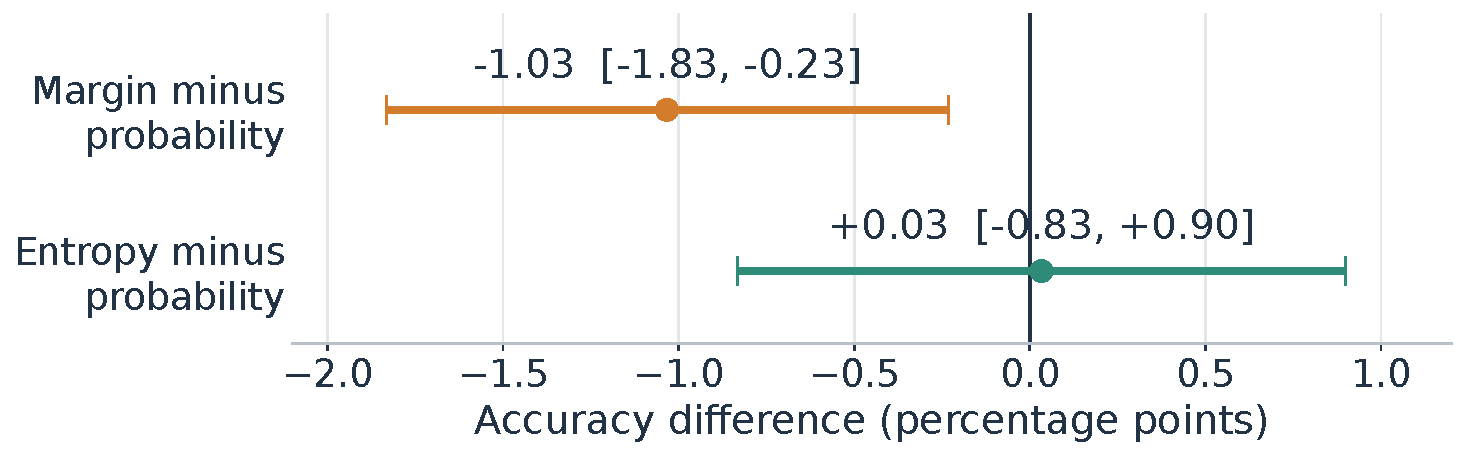
\includegraphics[width=0.95\linewidth,height=0.49\textheight,keepaspectratio]{adaptive_contrasts.pdf}
    \end{center}
    \begin{itemize}
        \item Margin has a small overall disadvantage.
        H2's ambiguity-specific claim remains untested.
        \item Entropy has no established advantage for H3.
    \end{itemize}

\end{frame}

\begin{frame}{Digit selection changes accuracy even with the same ordering rule}
    \begin{columns}[c,onlytextwidth]
        \begin{column}{0.65\textwidth}
            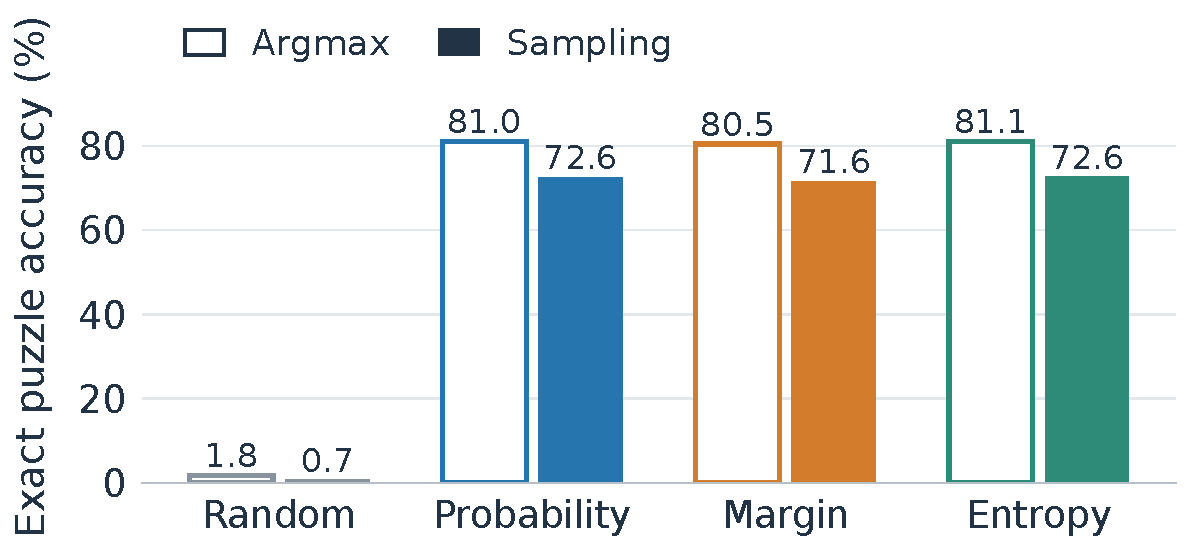
\includegraphics[width=\linewidth]{argmax_sampling.pdf}
        \end{column}
        \begin{column}{0.31\textwidth}
            \textbf{Argmax}
            \[\widehat{x}_i=\arg\max_j p_i(j).\]
            \textbf{Sampling}
            \[\widehat{x}_i\sim\mathrm{Cat}(p_i).\]
        \end{column}
    \end{columns}

\end{frame}

\begin{frame}{Constant raw-score noise sharply reduces accuracy}
    \begin{columns}[c,onlytextwidth]
        \begin{column}{0.61\textwidth}
            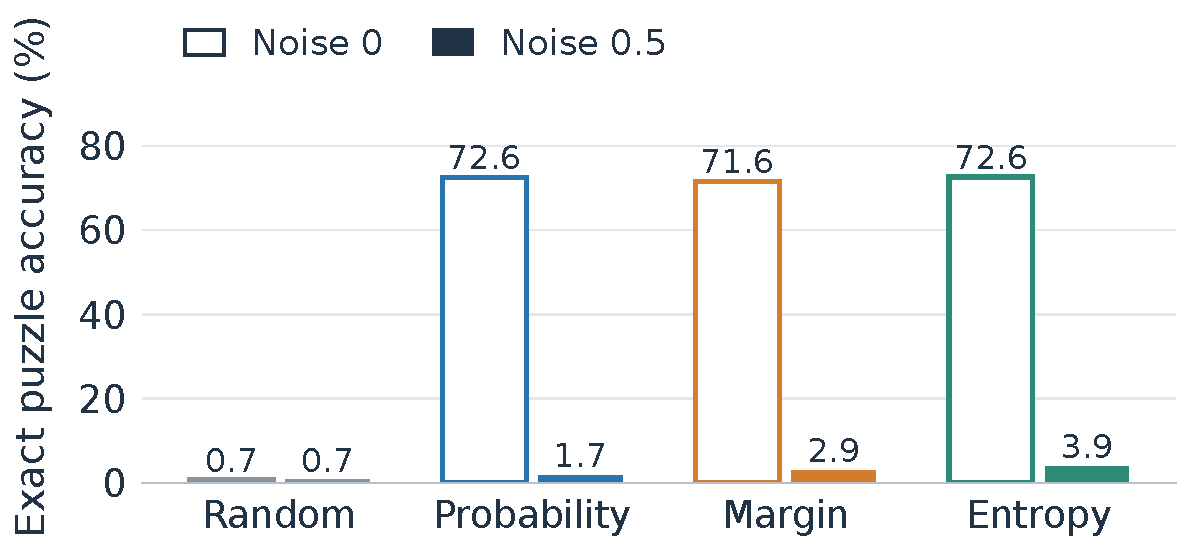
\includegraphics[width=\linewidth]{noise_accuracy.pdf}
        \end{column}
        \begin{column}{0.35\textwidth}
            \small
            \[\begin{gathered}
                \widetilde{s}_i=s_i+0.5G_i,\\
                G_i\sim\mathrm{Gumbel}(0,1).
            \end{gathered}\]
        \end{column}
    \end{columns}
\end{frame}

\begin{frame}{Adaptive ordering also helps every tested checkpoint}
    \begin{center}
        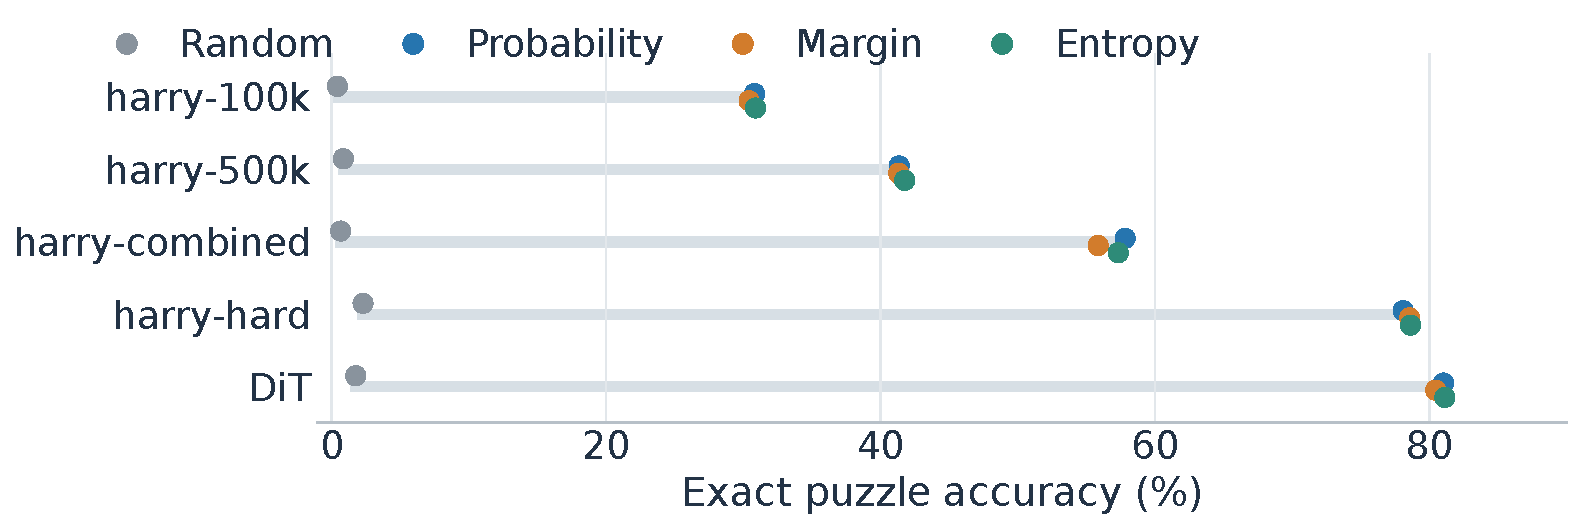
\includegraphics[width=0.96\linewidth,height=0.61\textheight,keepaspectratio]{checkpoint_accuracy.pdf}
    \end{center}
\end{frame}

\begin{frame}{Ordering matters most, while inference choices shape the result}
    \begin{enumerate}
        \item \textbf{Ordering has a large effect.}
        Adaptive rules greatly outperform random ordering.
        \medskip
        \item \textbf{Extra complexity brings no consistent gain.}
        Probability and entropy have similar means. Margin does not consistently win.
        \medskip
        \item \textbf{Implementation choices matter.}
        Digit sampling and constant raw-score noise substantially change accuracy.
    \end{enumerate}
    \medskip
    \condition{\url{https://github.com/Brixfoly/GM-project}}
\end{frame}

\end{document}
